\documentclass[12pt]{article}
\usepackage[top=0.75in, bottom=0.75in, left=0.75in, right=0.75in]{geometry}
\usepackage{amsmath, amssymb}
\usepackage{booktabs}
\usepackage{array}
\usepackage{enumitem}
\usepackage{graphicx}
\usepackage{float}
\usepackage{titlesec}
\usepackage{changepage}
\usepackage{color}
\usepackage{hyperref}

% Section numbering hierarchy
\renewcommand{\thesection}{\arabic{section}}
\renewcommand{\thesubsection}{(\arabic{subsection})}
\renewcommand{\thesubsubsection}{(\alph{subsubsection})}
\renewcommand{\theparagraph}{(\roman{paragraph})}
\setcounter{secnumdepth}{4}

% Make \paragraph behave like a numbered display-level heading.
\makeatletter
\renewcommand\paragraph{\@startsection{paragraph}{4}{\z@}%
    {-2.5ex\@plus -1ex \@minus -.25ex}%
    {1ex \@plus .2ex}%
    {\normalfont\normalsize\bfseries}}
\makeatother

%Heading indentation (escalates by level)
\titlespacing*{\section}      {0pt}     {*3}   {*1}
\titlespacing*{\subsection}   {1.5em}   {*2}   {*1}
\titlespacing*{\subsubsection}{3em}     {*1.5} {*0.8}
\titlespacing*{\paragraph}    {4.5em}   {*1}   {*0.5}

% Body-content indentation
\newenvironment{bodyL2}{\begin{adjustwidth}{3em}{0pt}}{\end{adjustwidth}}
\newenvironment{bodyL3}{\begin{adjustwidth}{4.5em}{0pt}}{\end{adjustwidth}}
\newenvironment{bodyL4}{\begin{adjustwidth}{6em}{0pt}}{\end{adjustwidth}}

% Graphics path
\graphicspath{{./}{./LP_baseline_output/}{./GPR_shock_output/}{./figures/}}

\title{GPR Shock Extraction and Baseline Local Projection \\ \large Summary Report}
\author{}
\date{\today}

\begin{document}
\maketitle

% ============================================================
\section{Overview}
% ============================================================

This report summarizes the construction of
\textcolor{blue}{\textbf{standardized geopolitical risk (GPR) shocks}} and their
use as impulses in a
\textcolor{blue}{\textbf{baseline local projection (LP) model}} to estimate the
dynamic response of oil-market prices and aggregate macro outcomes.
\\

The pipeline consists of three stages:

\begin{enumerate}[label=(\roman*), leftmargin=*]
\item \textbf{AR-residual extraction of standardized GPR shocks $z_t$}
      for three GPR series:
      \texttt{LGPR} (World), \texttt{LGPRT} (threats), \texttt{LGPRA} (acts).
      Two control specifications:

\begin{center}
\renewcommand{\arraystretch}{1.15}
\begin{tabular}{llcc}
\toprule
Regressor block & Timing & \texttt{w/ oil} & \texttt{w/o oil} \\
\midrule
GPR own lags                          & $t-1, \ldots, t-4$ & \checkmark & \checkmark \\
\texttt{Unemp}, \texttt{FFR}          & contemporaneous ($t$) & \checkmark & \checkmark \\
\texttt{Real\_Brent}, \texttt{Real\_WTI}, \texttt{Real\_Gasoline} & lag-1 ($t-1$) & \checkmark & --- \\
\bottomrule
\end{tabular}
\end{center}

%---------------------------------------------------------------
\item \textbf{Three diagnostic tests on $z_t$ to verify identification}:

\begin{center}
\renewcommand{\arraystretch}{1.15}
\begin{tabular}{clllr}
\toprule
\# & Test                         & Tool             & Lag(s)        & $N_{\text{tests}}$ \\
\midrule
1  & Conditional Granger exogeneity & \texttt{gctest}  & 4             & 30 \\
2  & Ljung-Box Q white noise        & \texttt{lbqtest} & $\{4,8,12\}$  & 18 \\
3  & Breusch-Godfrey LM (robust)    & aux.\ regression & $\{4,8,12\}$  & 18 \\
\bottomrule
\end{tabular}
\end{center}
$N_{\text{tests}}$: total tests run.
Test 1 $= 2 \text{ variants} \times 3 \text{ shocks} \times 5 \text{ predictors} = 30$;
Tests 2--3 $= 2 \times 3 \times 3 \text{ lag horizons} = 18$ each.

%---------------------------------------------------------------
\item \textbf{Local projection on $z_t$ for six outcome variables}.
      Settings: $H = 12$ quarters, 90\% Newey--West HAC bands, bandwidth $h + 1$.

\begin{center}
\renewcommand{\arraystretch}{1.15}
\begin{tabular}{ll}
\toprule
Block      & Variables \\
\midrule
Oil prices & \texttt{Real\_Brent}, \texttt{Real\_WTI}, \texttt{Real\_Gasoline} \\
Macro      & \texttt{Headline\_Pi}, \texttt{Core\_Pi}, \texttt{Indu\_Prod} \\
\bottomrule
\end{tabular}
\end{center}

\end{enumerate}

% ============================================================
\section{Data}
% ============================================================

\subsection{Source}
\begin{bodyL2}
\begin{itemize}[label=$\bullet$, leftmargin=*]
    \item File: \texttt{Q\_Levels\_Database.csv}
    \item Frequency: quarterly ($T = 160$ obs)
\end{itemize}
\end{bodyL2}

\subsection{Variables}
\begin{bodyL2}
\begin{center}
\renewcommand{\arraystretch}{1.15}
\begin{tabular}{lllll}
\toprule
Code & Definition & Role & Form & Source \\
\midrule
\texttt{LGPR}             & World GPR index           & shock target           & log               & TBD \\
\texttt{LGPRT}            & GP threats sub-index      & shock target           & log               & TBD \\
\texttt{LGPRA}            & GP acts sub-index         & shock target           & log               & TBD \\
\midrule
\texttt{Unemp}            & US unemployment rate      & control ($t$)          & rate              & TBD \\
\texttt{FFR}              & federal funds rate        & control ($t$)          & rate              & TBD \\
\midrule
\texttt{Real\_Brent}      & real Brent price          & control ($t{-}1$) + $y$ & real (CPI-defl.)  & TBD \\
\texttt{Real\_WTI}        & real WTI price            & control ($t{-}1$) + $y$ & real (CPI-defl.)  & TBD \\
\texttt{Real\_Gasoline}   & real gasoline price       & control ($t{-}1$) + $y$ & real (CPI-defl.)  & TBD \\
\midrule
\texttt{Headline\_Pi}     & headline CPI              & LP outcome ($y$)       & CPI inflation     & TBD \\
\texttt{Core\_Pi}         & core CPI                  & LP outcome ($y$)       & CPI inflation     & TBD \\
\texttt{Indu\_Prod}       & industrial production     & LP outcome ($y$)       & TBD               & TBD \\
\bottomrule
\end{tabular}
\end{center}

\bigskip
\textbf{Note:} To be double-checked!
\begin{itemize}
    \item[--] \textbf{\texttt{LGPR}, \texttt{LGPRT}, \texttt{LGPRA}}: codebook says
          ``log'', but 1986Q1 value $\approx 470$ matches $100 \times \ln(\text{GPR})$ for raw GPR $\approx 110$ (not $\ln(\text{GPR}) \approx 4.7$).
          Likely $100 \times \log$ in practice.
    \item[--] \textbf{\texttt{Headline\_Pi}, \texttt{Core\_Pi}}: codebook says
          ``CPI inflation'', but 1986Q1 value $\approx 470$ matches $100 \times \ln(\text{CPI level})$, not an inflation rate (which would be $1$--$5\%$).
\end{itemize}
\end{bodyL2}

\subsection{Sample window}
\begin{bodyL2}
All available observations are used. \textbf{The binding constraint is the late start of
\texttt{Real\_Brent} (first non-missing 1987Q3)}.

\begin{center}
\renewcommand{\arraystretch}{1.15}
\begin{tabular}{lr}
\toprule
Stage & $n$ \\
\midrule
Raw quarterly data (1986Q1--2025Q4)            & 160 \\
After AR($p = 4$) lag truncation               & 156 \\
\midrule
Shock sample, \texttt{w/ oil}                    & \textbf{153} \\
Shock sample, \texttt{w/o oil}                 & \textbf{156} \\
\midrule
LP sample at $h = 0$, $y \in$ \{\texttt{WTI}, \texttt{Gas}\}    & 153 \\
LP sample at $h = 0$, $y \in$ \{\texttt{Brent}, macro\}         & 150 \\
LP sample at horizon $h$                       & (above) $- h$ \\
\bottomrule
\end{tabular}
\end{center}

\smallskip
\textbf{Note:}
\begin{itemize}
    \item[--] \texttt{w/ oil} loses 3 extra obs: needs lag-1 Brent at $t = 5,6,7$, missing.
    \item[--] LP needing Brent at $t-1,\ldots,t-4$ starts at $t = 11$ (1988Q3) $\Rightarrow$ 150 rows.
    \item[--] LP at horizon $h$ loses $h$ end-of-sample rows ($t + h \le T$).
\end{itemize}
\end{bodyL2}

\subsection{Oil-price multicollinearity}
\begin{bodyL2}
Pairwise correlations of the three lag-1 oil controls:

\begin{center}
\begin{tabular}{lccc}
\toprule
                        & \texttt{Real\_Brent} & \texttt{Real\_WTI} & \texttt{Real\_Gasoline} \\
\midrule
\texttt{Real\_Brent}    & 1.000 & 0.993 & 0.976 \\
\texttt{Real\_WTI}      & 0.993 & 1.000 & 0.973 \\
\texttt{Real\_Gasoline} & 0.976 & 0.973 & 1.000 \\
\bottomrule
\end{tabular}
\end{center}

\smallskip
$\Rightarrow$ Correlations of $0.97$--$0.99$ flag substantial multicollinearity.
\end{bodyL2}

% ============================================================
\section{GPR Shock Extraction}
\label{sec:shock}
% ============================================================

\subsection{AR specification}
\begin{bodyL2}
For each GPR series the standardized shock $z_t$ is the OLS residual of
\begin{equation}
    \text{GPR}_t
    = a
    + \sum_{j=1}^{p} \rho_j\, \text{GPR}_{t-j}
    + \xi'\, B_t
    + \omega'\, O_{t-1}
    + u_t,
    \qquad
    z_t = \frac{u_t - \bar u}{s_u},
    \label{eq:shock}
\end{equation}
with $p = 4$, $B_t = [\text{Unemp}_t, \text{FFR}_t]$, and
$O_{t-1} = [\text{Brent}, \text{WTI}, \text{Gas}]_{t-1}$.
\end{bodyL2}

\subsection{Identifying logic for control timing}
\begin{bodyL2}
\begin{center}
\renewcommand{\arraystretch}{1.2}
\begin{tabular}{llp{2.6in}}
\toprule
Controls & Timing & Reason \\
\midrule
\texttt{Unemp}, \texttt{FFR}                & contemporaneous ($t$) & slow-moving; no bad-control bias \\
\texttt{Brent}, \texttt{WTI}, \texttt{Gas}  & lag-1 ($t-1$)         & contemporaneous use would partial out the transmission channel \\
\bottomrule
\end{tabular}
\end{center}
\end{bodyL2}

\subsection{Shock-extraction summary}
\begin{bodyL2}
\begin{center}
\begin{tabular}{llrrrr}
\toprule
Variant          & Shock & nobs & AR $R^2$ & Resid sd & $\mathrm{cond}(X'X)$ \\
\midrule
\texttt{w/ oil}    & World & 153 & 0.507 & 22.96 & $5.6 \times 10^{9}$ \\
\texttt{w/ oil}    & GPT   & 153 & 0.515 & 22.58 & $5.8 \times 10^{9}$ \\
\texttt{w/ oil}    & GPA   & 153 & 0.538 & 30.44 & $5.4 \times 10^{9}$ \\
\midrule
\texttt{w/o oil} & World & 156 & 0.505 & 22.79 & $2.9 \times 10^{8}$ \\
\texttt{w/o oil} & GPT   & 156 & 0.512 & 22.45 & $3.2 \times 10^{8}$ \\
\texttt{w/o oil} & GPA   & 156 & 0.529 & 30.43 & $1.4 \times 10^{8}$ \\
\bottomrule
\end{tabular}
\end{center}
\end{bodyL2}

\subsection{Takeaways}
\begin{bodyL2}
\begin{itemize}
    \item \textbf{Specification robust}: $\Delta R^2 < 0.01$, $\Delta\text{sd} < 0.2$ across variants.
    \item \textbf{Two shocks essentially identical}.
    \item \textbf{Oil controls inflate $\mathrm{cond}(X'X)$ by $\sim 20\times$}, still well below $10^{12}$.
    \item \textbf{Multicollinearity is benign for the residual}: residual depends on the column space, not on individual columns.
\end{itemize}
\end{bodyL2}

% ============================================================
\section{Shock Validation Diagnostics}
% ============================================================

\subsection{Test 1 --- Conditional Granger exogeneity}
\begin{bodyL3}
\begin{itemize}
    \item $H_0$: lagged $X_j$ does not Granger-cause $z_t$, conditional on lags of the
    other four predictors in $\{\texttt{Unemp}, \texttt{FFR}, \texttt{Real\_Brent}, \texttt{Real\_WTI}, \texttt{Real\_Gasoline}\}$.
    \item Tool: \texttt{gctest} with $L = 4$.
    \item \textbf{Results} (30 tests $= 2$ variants $\times 3$ shocks $\times 5$ predictors):
\end{itemize}

\begin{center}
\renewcommand{\arraystretch}{1.15}
\begin{tabular}{lcc}
\toprule
Variant      & Rejections at $\alpha = 0.05$ & Smallest $p$ \\
\midrule
\texttt{w/ oil}    & 1 / 15 (\texttt{FFR} $\to z_{\text{GPA}}$, $p = 0.032$) & 0.032 \\
\texttt{w/o oil} & 0 / 15                                                  & 0.065 \\
\midrule
Combined         & 1 / 30                                                  & 0.032 \\
\bottomrule
\end{tabular}
\end{center}

\smallskip
\begin{itemize}
    \item[--] 28 of 30 $p$-values exceed 0.10.
    \item[--] Expected false positives at $\alpha = 0.05$: 1.5 $\Rightarrow$ 1 rejection within chance.
    \item[--] \underline{\textbf{Bonferroni ($\alpha = 0.05/30 \approx 0.0017$): 0 rejections.}}
    \item[--] \textbf{Conclusion}: \underline{\textbf{shocks are exogenous to past macro/oil-price information.}}
\end{itemize}
\end{bodyL3}

\subsection{Test 2 --- Ljung-Box Q (white noise)}
\begin{bodyL3}
\begin{itemize}
    \item $H_0$: $z_t$ is white noise (no serial correlation up to lag $L$). \item Tool: \texttt{lbqtest}.
    \item \textbf{Results} (18 tests $= 2 \times 3 \times 3$):
\end{itemize}

\begin{center}
\renewcommand{\arraystretch}{1.15}
\begin{tabular}{lcc}
\toprule
Rejections & Min $p$-value & Conclusion \\
\midrule
0 / 18 & $0.798$ & no serial correlation \\
\bottomrule
\end{tabular}
\end{center}
\end{bodyL3}

\subsection{Test 3 --- Breusch-Godfrey LM (robustness)}
\begin{bodyL3}
\begin{itemize}
    \item $H_0$: $\gamma_1 = \cdots = \gamma_L = 0$ in
\[
    z_t = X_t'\alpha + \sum_{k=1}^{L}\gamma_k\, z_{t-k} + v_t,
    \qquad
    \mathrm{LM} = n R^2_{\text{aux}} \xrightarrow{d} \chi^2(L).
\]
$X_t$ = original AR$(p)$ regressors.
    \item Preferred over LBQ when lagged dependent variables enter the regression (our case).
    \item \textbf{Results} (18 tests):


\begin{center}
\renewcommand{\arraystretch}{1.15}
\begin{tabular}{lcc}
\toprule
Rejections & Min LM $p$-value & Conclusion \\
\midrule
0 / 18 & $0.319$ & no serial correlation (robust) \\
\bottomrule
\end{tabular}
\end{center}

\item BG $p$-values are systematically lower than LBQ (BG partials out the original
regressors) but lead to the same conclusion.
\end{itemize}
\end{bodyL3}

\subsection{Summary of diagnostics}
\begin{bodyL2}
\begin{center}
\renewcommand{\arraystretch}{1.3}
\begin{tabular}{llll}
\toprule
Test & Rejections & Min $p$ & Conclusion \\
\midrule
1. Conditional Granger & 1 / 30 (borderline) & 0.032 & shocks exogenous \\
2. Ljung-Box Q         & 0 / 18              & 0.798 & no serial correlation \\
3. Breusch-Godfrey LM  & 0 / 18              & 0.319 & confirmed (robust) \\
\bottomrule
\end{tabular}
\end{center}
\end{bodyL2}

\subsection{Face validity --- event alignment of $z_t$}

\begin{figure}[H]
    \centering
    \includegraphics[width=\linewidth]{z_shocks_timeseries.png}
    \caption{Standardized GPR shocks $z_t$ over 1986Q1--2025Q4}
    \label{fig:z_timeseries}
\end{figure}

\smallskip
$\Rightarrow$ \textbf{Spike alignment with major events} (\texttt{w/ oil} variant $z_t$ values):

\begin{center}
\renewcommand{\arraystretch}{1.15}
\begin{tabular}{llrrr}
\toprule
Event                       & Quarter & World          & GPT (threats)  & GPA (acts) \\
\midrule
Gulf War (Iraq--Kuwait)     & 1990Q3  & $+3.23$        & $\mathbf{+4.32}$ & $+1.16$ \\
9/11                        & 2001Q3  & $\mathbf{+4.83}$ & $+2.51$        & $\mathbf{+5.27}$ \\
Iraq War                    & 2003Q1  & $+2.69$        & $+3.48$        & $+1.93$ \\
Crimea annexation           & 2014Q1  & $+0.39$        & $+0.68$        & $-0.13$ \\
Russia--Ukraine             & 2022Q1  & $+3.70$        & $+4.29$        & $+2.54$ \\
Israel--Hamas               & 2023Q4  & $+1.88$        & $+1.22$        & $+2.46$ \\
\bottomrule
\end{tabular}
\end{center}
(Sample max in bold per column.)

\smallskip
$\Rightarrow$ \textbf{Observations:}
\begin{itemize}
    \item All major events except Crimea produce positive $z_t$ spikes; magnitudes broadly scale with event size.
    \item \texttt{w/ oil} (blue) and \texttt{w/o oil} (red) lines are visually indistinguishable (the spec-robustness claim).
    \item \textbf{Sample maxima}: 9/11 dominates World and GPA (4.83 and 5.27); Gulf War dominates GPT (4.32, with Russia--Ukraine 4.29 essentially tied).
    \item The 2014 Crimea annexation barely registers, possibly because the annexation was a contained event with limited global escalation at the time.
\end{itemize}

\begin{center}
\boxed{
    \begin{minipage}{0.9\linewidth}
        \centering
        $\Rightarrow$ \textbf{Conclusion}: $z_t$ is not only statistically white noise but also carries \textbf{economically meaningful information} about geopolitical events.
    \end{minipage}
}
\end{center}


% ============================================================
\section{Baseline LP Model}
\label{sec:lp}
% ============================================================

\subsection{Specification}
\begin{bodyL2}
For each shock $z_t$ and outcome $y$, at horizon $h = 0, 1, \ldots, H$:
\begin{equation}
    y_{t+h} - y_{t-1}
    = \alpha_h
    + \beta_h\, z_t
    + \sum_{j=1}^{p} \rho_{h,j}\, y_{t-j}
    + \sum_{j=1}^{p} \gamma_{h,j}\, \text{GPR}_{t-j}
    + \sum_{j=1}^{p} \theta_{h,j}'\, \text{controls}_{t-j}
    + e_{t+h}.
    \label{eq:lp}
\end{equation}
\end{bodyL2}

\subsection{Settings}
\begin{bodyL2}
\begin{center}
\renewcommand{\arraystretch}{1.15}
\begin{tabular}{ll}
\toprule
Setting & Value \\
\midrule
Lag length      & $p = 4$ (matches AR shock extraction) \\
Horizon         & $h = 0, \ldots, H = 12$ quarters \\
Shock size      & 1 s.d. (since $z_t$ is standardized) \\
Inference       & Newey--West HAC, Bartlett kernel, bandwidth $= h + 1$ \\
Confidence band & $90\%$ \\
\bottomrule
\end{tabular}
\end{center}
\end{bodyL2}

\subsection{Outcome-dependent control set}
\begin{bodyL2}
To avoid SE inflation from oil-price multicollinearity, the full control pool is pruned dynamically based on the outcome variable:

\begin{center}
\renewcommand{\arraystretch}{1.3}
\small
\begin{tabular}{p{2.5in} p{3.5in}}
\toprule
Outcome ($y$) & Control Variables \\
\midrule
\textbf{Oil price} \newline (any of \texttt{Real\_Brent/WTI/Gasoline})
  & \texttt{Unemp}, \texttt{FFR}, \texttt{Headline\_Pi}, \texttt{Core\_Pi}, \texttt{Indu\_Prod} \\
\midrule
\texttt{Headline\_Pi}
  & \texttt{Unemp}, \texttt{FFR}, \texttt{Real\_Brent}, \texttt{Real\_WTI}, \texttt{Real\_Gasoline}, \texttt{Core\_Pi}, \texttt{Indu\_Prod} \\
\midrule
\texttt{Core\_Pi}
  & \texttt{Unemp}, \texttt{FFR}, \texttt{Real\_Brent}, \texttt{Real\_WTI}, \texttt{Real\_Gasoline}, \texttt{Headline\_Pi}, \texttt{Indu\_Prod} \\
\midrule
\texttt{Indu\_Prod}
  & \texttt{Unemp}, \texttt{FFR}, \texttt{Real\_Brent}, \texttt{Real\_WTI}, \texttt{Real\_Gasoline}, \texttt{Headline\_Pi}, \texttt{Core\_Pi} \\
\bottomrule
\end{tabular}
\end{center}
\end{bodyL2}


% ============================================================
\section{Results}
% ============================================================

\subsection{Shock-specification robustness}
\begin{bodyL2}
Across all 18 panels (3 shocks $\times$ 6 outcomes), \texttt{w/ oil} and \texttt{w/o oil}
IRFs and bands are visually indistinguishable
(see Section~6-(6) for IRF figures).
\end{bodyL2}

\subsection{Oil-price peaks}
\begin{bodyL2}
Peak responses in the \texttt{w/ oil} variant (1 s.d.\ shock; positive = price rise; $H = 12$):

\begin{center}
\renewcommand{\arraystretch}{1.15}
\begin{tabular}{lcrrr|rr}
\toprule
                & & \multicolumn{3}{c}{Peak} & \multicolumn{2}{c}{$\beta_0$} \\
\cmidrule(lr){3-5} \cmidrule(l){6-7}
Shock & Outcome  & $\beta$ & $h$ & $t$    & $\beta$ & $t$ \\
\midrule
GPT   & Brent    & $+7.16$ & 7  & $3.27$ & $+2.66$ & $1.73$ \\
GPT   & WTI      & $+6.49$ & 7  & $3.17$ & $+2.40$ & $1.73$ \\
GPT   & Gasoline & $+3.11$ & 7  & $2.61$ & $+0.59$ & $0.92$ \\
\midrule
World & Brent    & $+4.55$ & 9  & $2.24$ & $+1.23$ & $0.74$ \\
World & WTI      & $+4.15$ & 9  & $2.27$ & $+0.94$ & $0.61$ \\
World & Gasoline & $+2.16$ & 9  & $1.95$ & $-0.14$ & $-0.19$ \\
\midrule
GPA   & Brent    & $+3.82$ & 9  & $2.19$ & $-0.75$ & $-0.61$ \\
GPA   & WTI      & $+3.75$ & 12 & $1.78$ & $-0.71$ & $-0.60$ \\
GPA   & Gasoline & $+1.97$ & 9  & $2.11$ & $-0.75$ & $-1.14$ \\
\bottomrule
\end{tabular}
\end{center}

\smallskip
\begin{itemize}[label=$\bullet$, leftmargin=*]
    \item \textbf{GPT (threats)}: short-horizon hump, peaks at $h = 7$. Strongest significance ($t \approx 3$).
    \item \textbf{World, GPA (acts)}: delayed peaks at $h \approx 9$--$12$, smaller magnitudes than GPT.
    \item \textbf{Peak significance}: 8 of 9 peaks clear $90\%$ ($|t| \ge 1.645$); only GPA$\to$WTI at $h=12$ is borderline ($t = 1.78$).
    \item \texttt{w/ oil} vs \texttt{w/o oil} differ by $< 0.5$ at peak (shock-spec robust).
\end{itemize}

\smallskip
\textbf{Caveat (pointwise significance across horizons).}
The peak rows above pick the single most-significant horizon. Across all
$h = 0, \ldots, 12$, the share of horizons clearing the $90\%$ band varies
considerably:

\begin{center}
\renewcommand{\arraystretch}{1.15}
\small
\begin{tabular}{lccc}
\toprule
Shock & Brent & WTI & Gasoline \\
\midrule
GPT   & 7 / 13 (54\%) & 7 / 13 (54\%) & 5 / 13 (38\%) \\
World & 5 / 13 (38\%) & 7 / 13 (54\%) & 4 / 13 (31\%) \\
GPA   & 1 / 13 (8\%)  & 3 / 13 (23\%) & 4 / 13 (31\%) \\
\bottomrule
\end{tabular}
\end{center}
$\Rightarrow$ The peak finding is real (at least one horizon is significant for
every cell), but \textbf{persistence across horizons is uneven}, especially for
GPA. Visual IRFs in Section~6-(6) show this directly: bands often contain zero
outside a short window around the peak.
\end{bodyL2}

\subsection{Inflation peaks}
\begin{bodyL2}
$y_{t+h} - y_{t-1}$ = cumulative \% change in CPI. Most-negative point estimates ($H = 12$):

\begin{center}
\renewcommand{\arraystretch}{1.15}
\begin{tabular}{ll rrr}
\toprule
Shock & Outcome & $\beta$ & $h$ & $t$ \\
\midrule
World & \texttt{Headline\_Pi} & $-0.131$ & 10 & $-0.99$ \\
World & \texttt{Core\_Pi}     & $-0.143$ & 12 & $-1.28$ \\
GPT   & \texttt{Headline\_Pi} & $-0.089$ & 12 & $-0.52$ \\
GPT   & \texttt{Core\_Pi}     & $-0.133$ & 12 & $-0.97$ \\
GPA   & \texttt{Headline\_Pi} & $-0.199$ & 10 & $-1.71$ \\
GPA   & \texttt{Core\_Pi}     & $-0.179$ & 10 & $-1.93$ \\
\bottomrule
\end{tabular}
\end{center}

\smallskip
\textbf{Pointwise significance across horizons} ($h = 0, \ldots, 12$):
\begin{center}
\renewcommand{\arraystretch}{1.15}
\small
\begin{tabular}{lcc}
\toprule
Shock & Headline\_Pi & Core\_Pi \\
\midrule
World & 0 / 13 (0\%)  & 0 / 13 (0\%) \\
GPT   & 0 / 13 (0\%)  & 0 / 13 (0\%) \\
GPA   & 4 / 13 (31\%) & 6 / 13 (46\%) \\
\bottomrule
\end{tabular}
\end{center}

\smallskip
\begin{itemize}[label=$\bullet$, leftmargin=*]
    \item Inflation responses to GPR shocks are largely
\textbf{statistically indistinguishable from zero}.
    \item \textbf{4 of 6 cells have 0 / 13 significant horizons} (World and GPT for both Headline and Core). The entire IRF stays within the $90\%$ band of zero.
    \item Only \texttt{GPA $\to$ Headline/Core} produce borderline signal (peak $t \approx -1.7$ to $-1.9$, 4--6 of 13 horizons significant), in the \textbf{negative} (deflationary) direction.
    \item Contemporaneous response $\approx 0$ everywhere: $|\beta_0| \le 0.06$ (headline), $|\beta_0| \le 0.02$ (core).
    \item The slide-deck's cost-push prior (``threats inflate, acts deflate'') is \textbf{not supported}: GPT shows no effect, and GPA points in the deflationary direction for both Headline and Core.
    \item \textbf{Interpretation}: Either
(i) the demand channel (uncertainty $\to$ contraction $\to$ disinflation)
dominates the cost-push channel; or
(ii) the macro block in the LP control set absorbs the cost-push channel
through lagged oil prices, leaving only the residual demand effect; or
(iii) the GPR-to-inflation spillover is too small relative to other macro
noise at the quarterly frequency to be detected with 153 observations.
\end{itemize}
\end{bodyL2}

\subsection{Industrial production peaks}
\begin{bodyL2}

\smallskip
\textbf{Most-significant horizon per shock} (\texttt{w/ oil} variant; $H = 12$):

\begin{center}
\renewcommand{\arraystretch}{1.15}
\begin{tabular}{l rrr l}
\toprule
Shock & $\beta$ & $h$ & $t$ & Note \\
\midrule
GPT   & $-0.007$ & 11 & $-1.50$ & $-0.7\%$, borderline ($p \approx 0.13$) \\
World & $-0.003$ & 11 & $-0.81$ & not significant \\
GPA   & $-0.003$ &  1 & $-1.80$ & $-0.3\%$, sig at 90\% (short-run only) \\
\bottomrule
\end{tabular}
\end{center}

\smallskip
\textbf{Pointwise significance across horizons} ($h = 0, \ldots, 12$):

\begin{center}
\renewcommand{\arraystretch}{1.15}
\small
\begin{tabular}{lc}
\toprule
Shock & \texttt{Indu\_Prod} \\
\midrule
World & 0 / 13 (0\%) \\
GPT   & 1 / 13 (8\%) \\
GPA   & 1 / 13 (8\%) \\
\bottomrule
\end{tabular}
\end{center}

\smallskip
\begin{itemize}[label=$\bullet$, leftmargin=*]
    \item IP responses are \textbf{even weaker than inflation}
--- the IRFs stay near zero with wide bands across almost all horizons.
    \item The same three explanations as for inflation apply,
plus a fourth: IP is even slower-moving than inflation, so a 12-quarter
horizon may simply be too short to detect macro spillover from GPR shocks.
\end{itemize}
\end{bodyL2}

\newpage
\begin{figure}[!htbp]
    \centering
    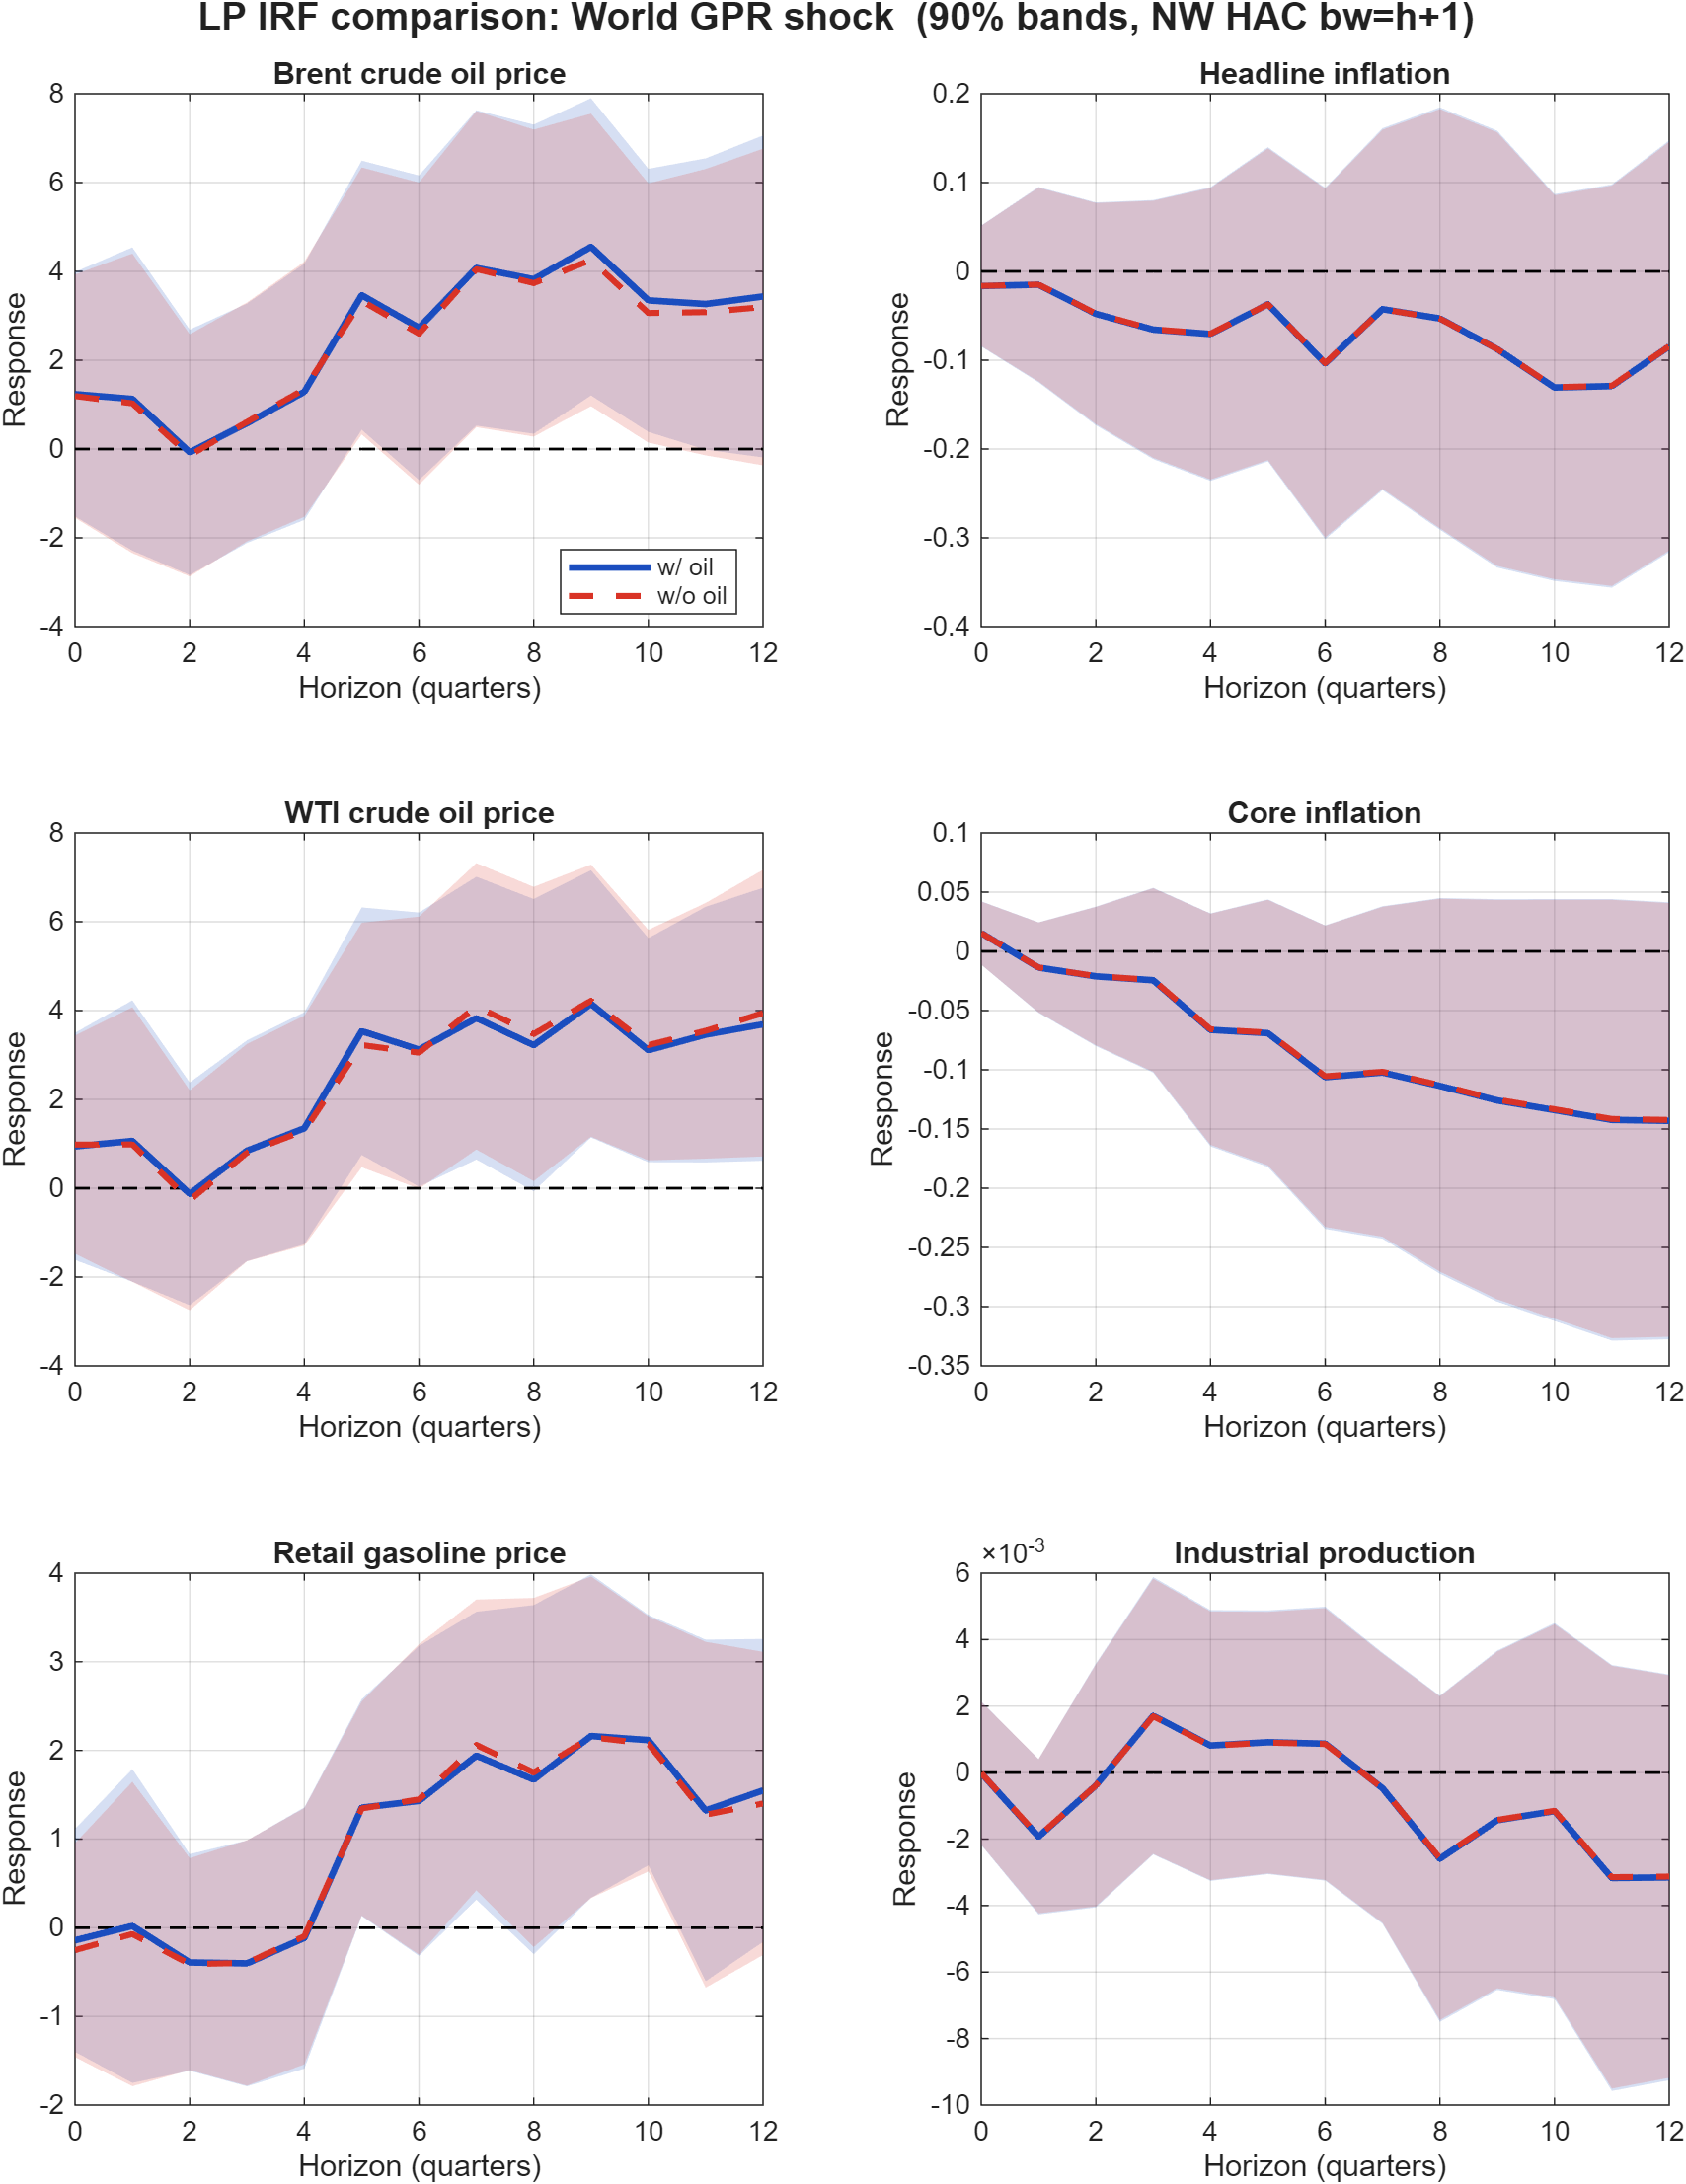
\includegraphics[width=\linewidth]{IRF_compare_World.png}
    \caption{IRF to a 1 s.d.\ World GPR shock.Shaded: 90\% NW HAC bands, bandwidth $h+1$.}
    \label{fig:irf_world}
\end{figure}

\begin{figure}[!htbp]
    \centering
    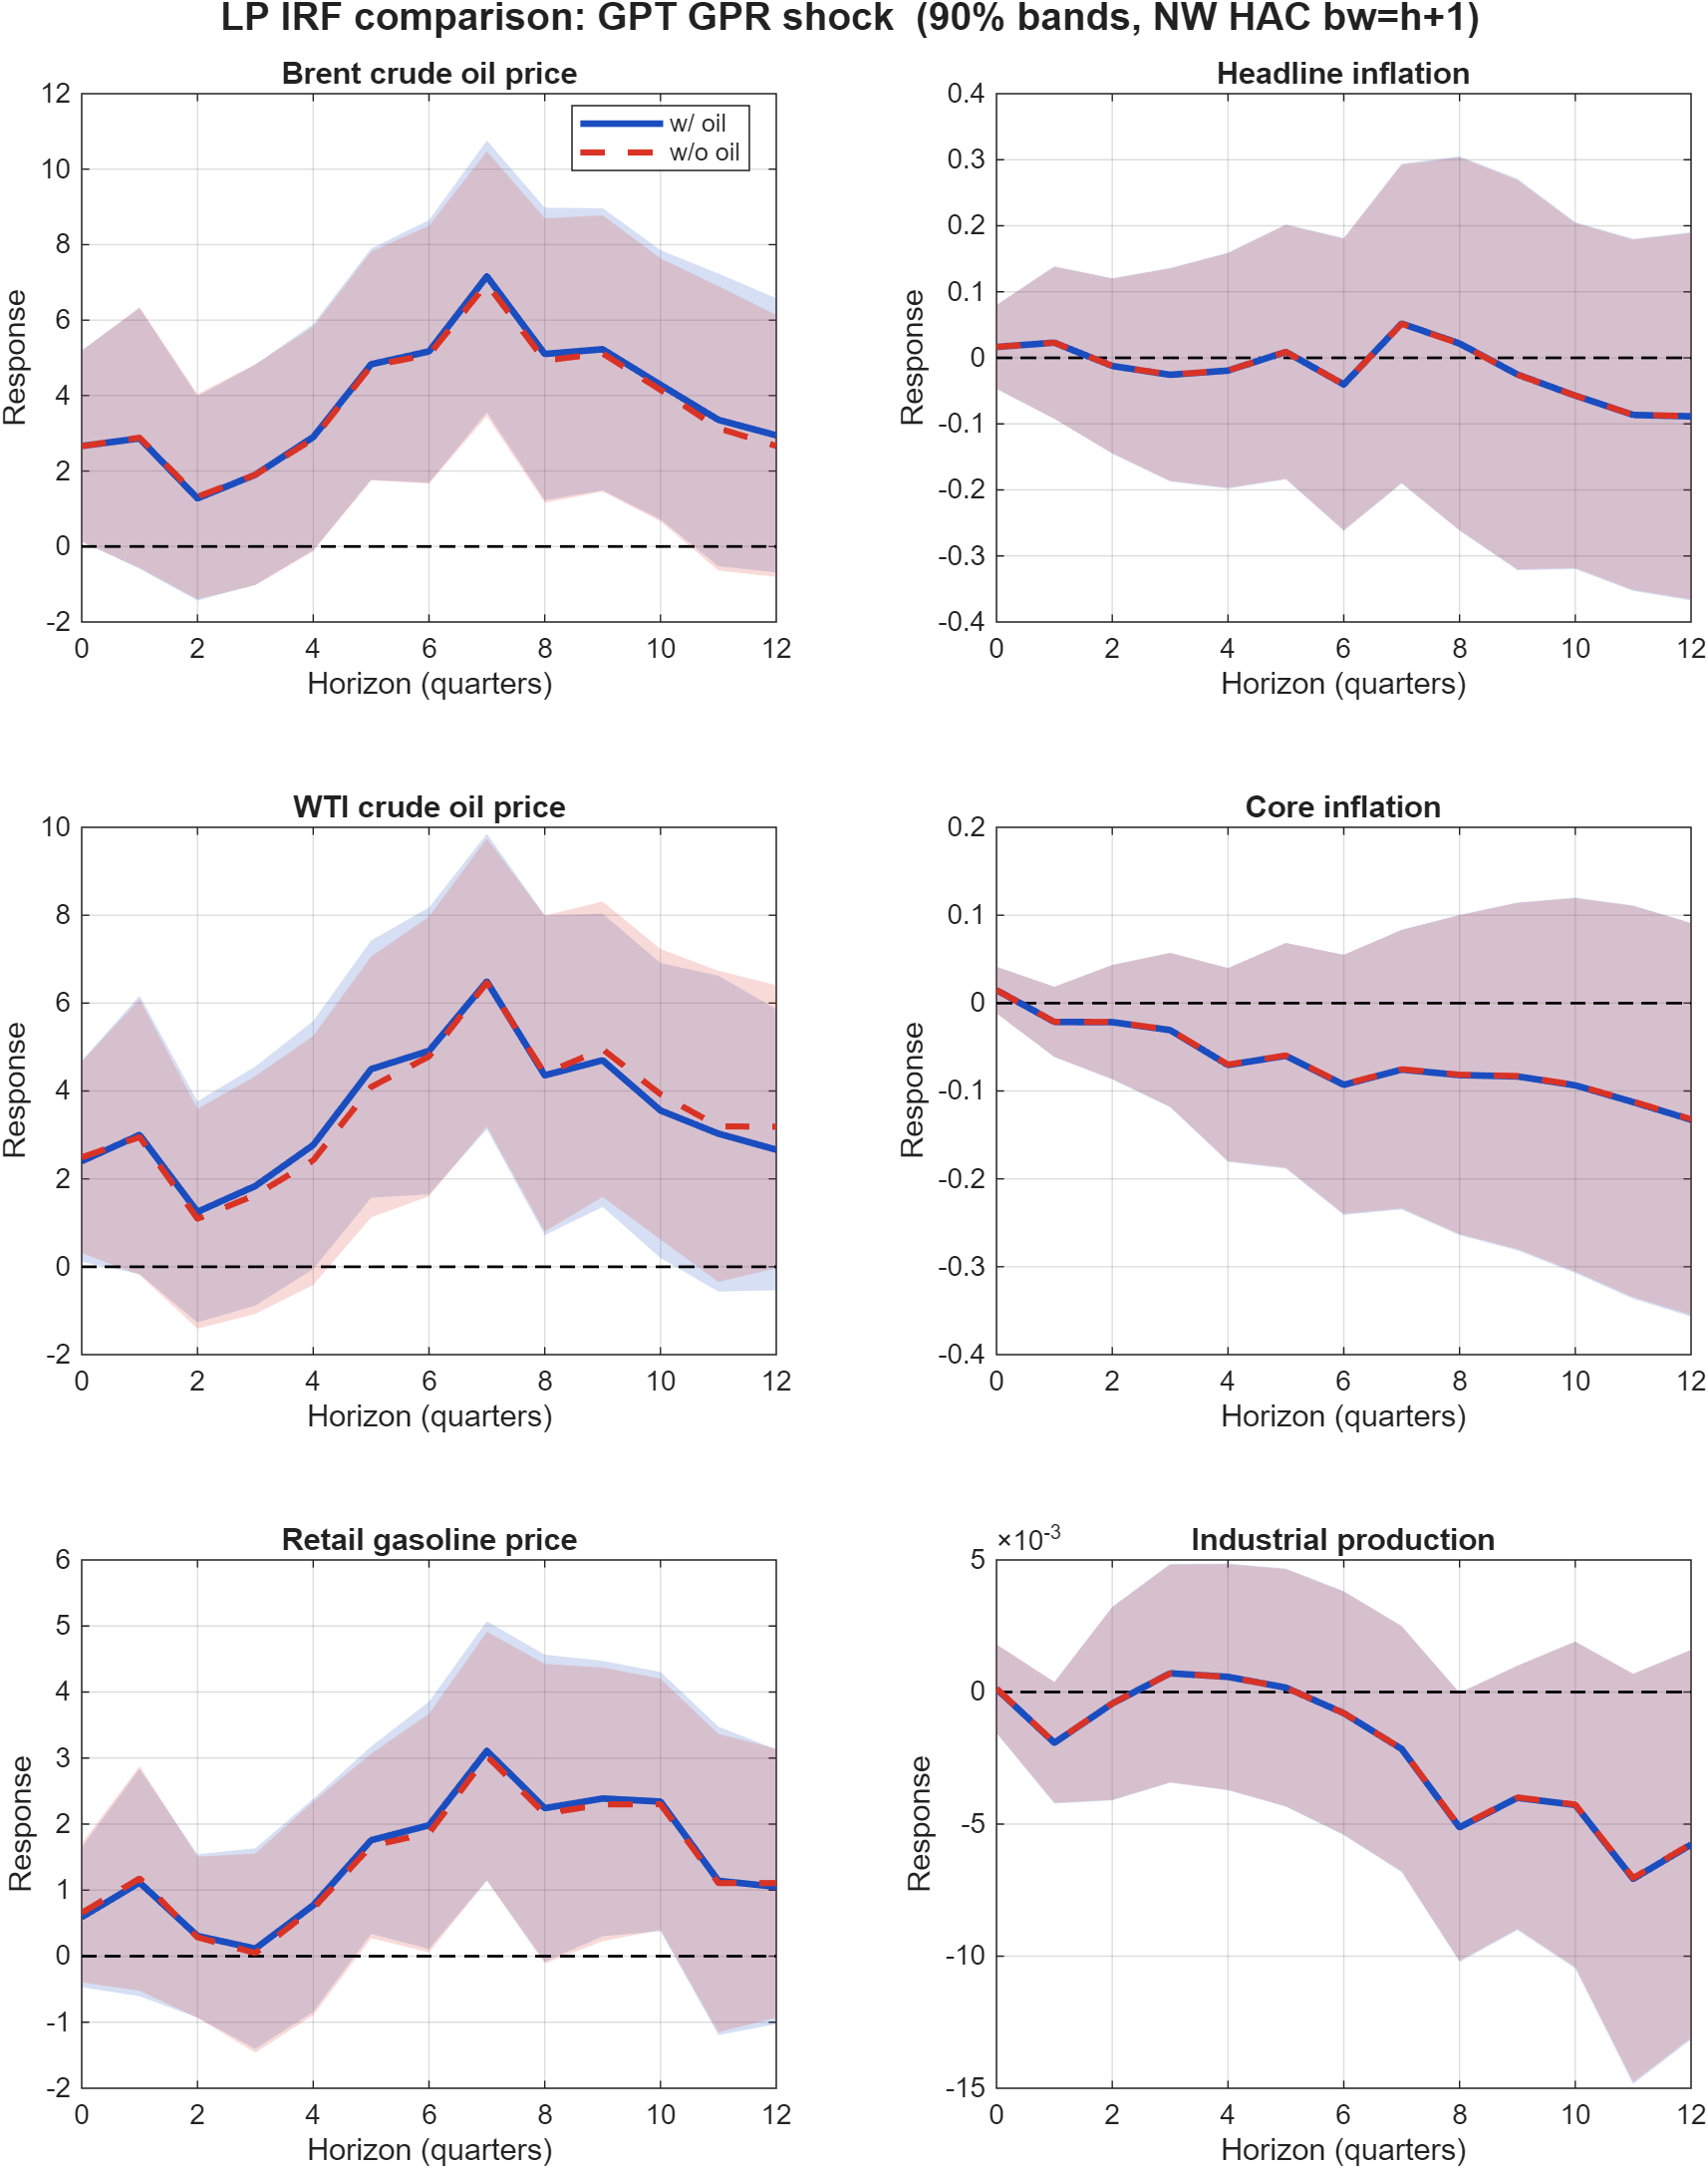
\includegraphics[width=\linewidth]{IRF_compare_GPT.png}
    \caption{IRF to a 1 s.d.\ GPT (threats) shock. Conventions as above.}
    \label{fig:irf_gpt}
\end{figure}

\begin{figure}[!htbp]
    \centering
    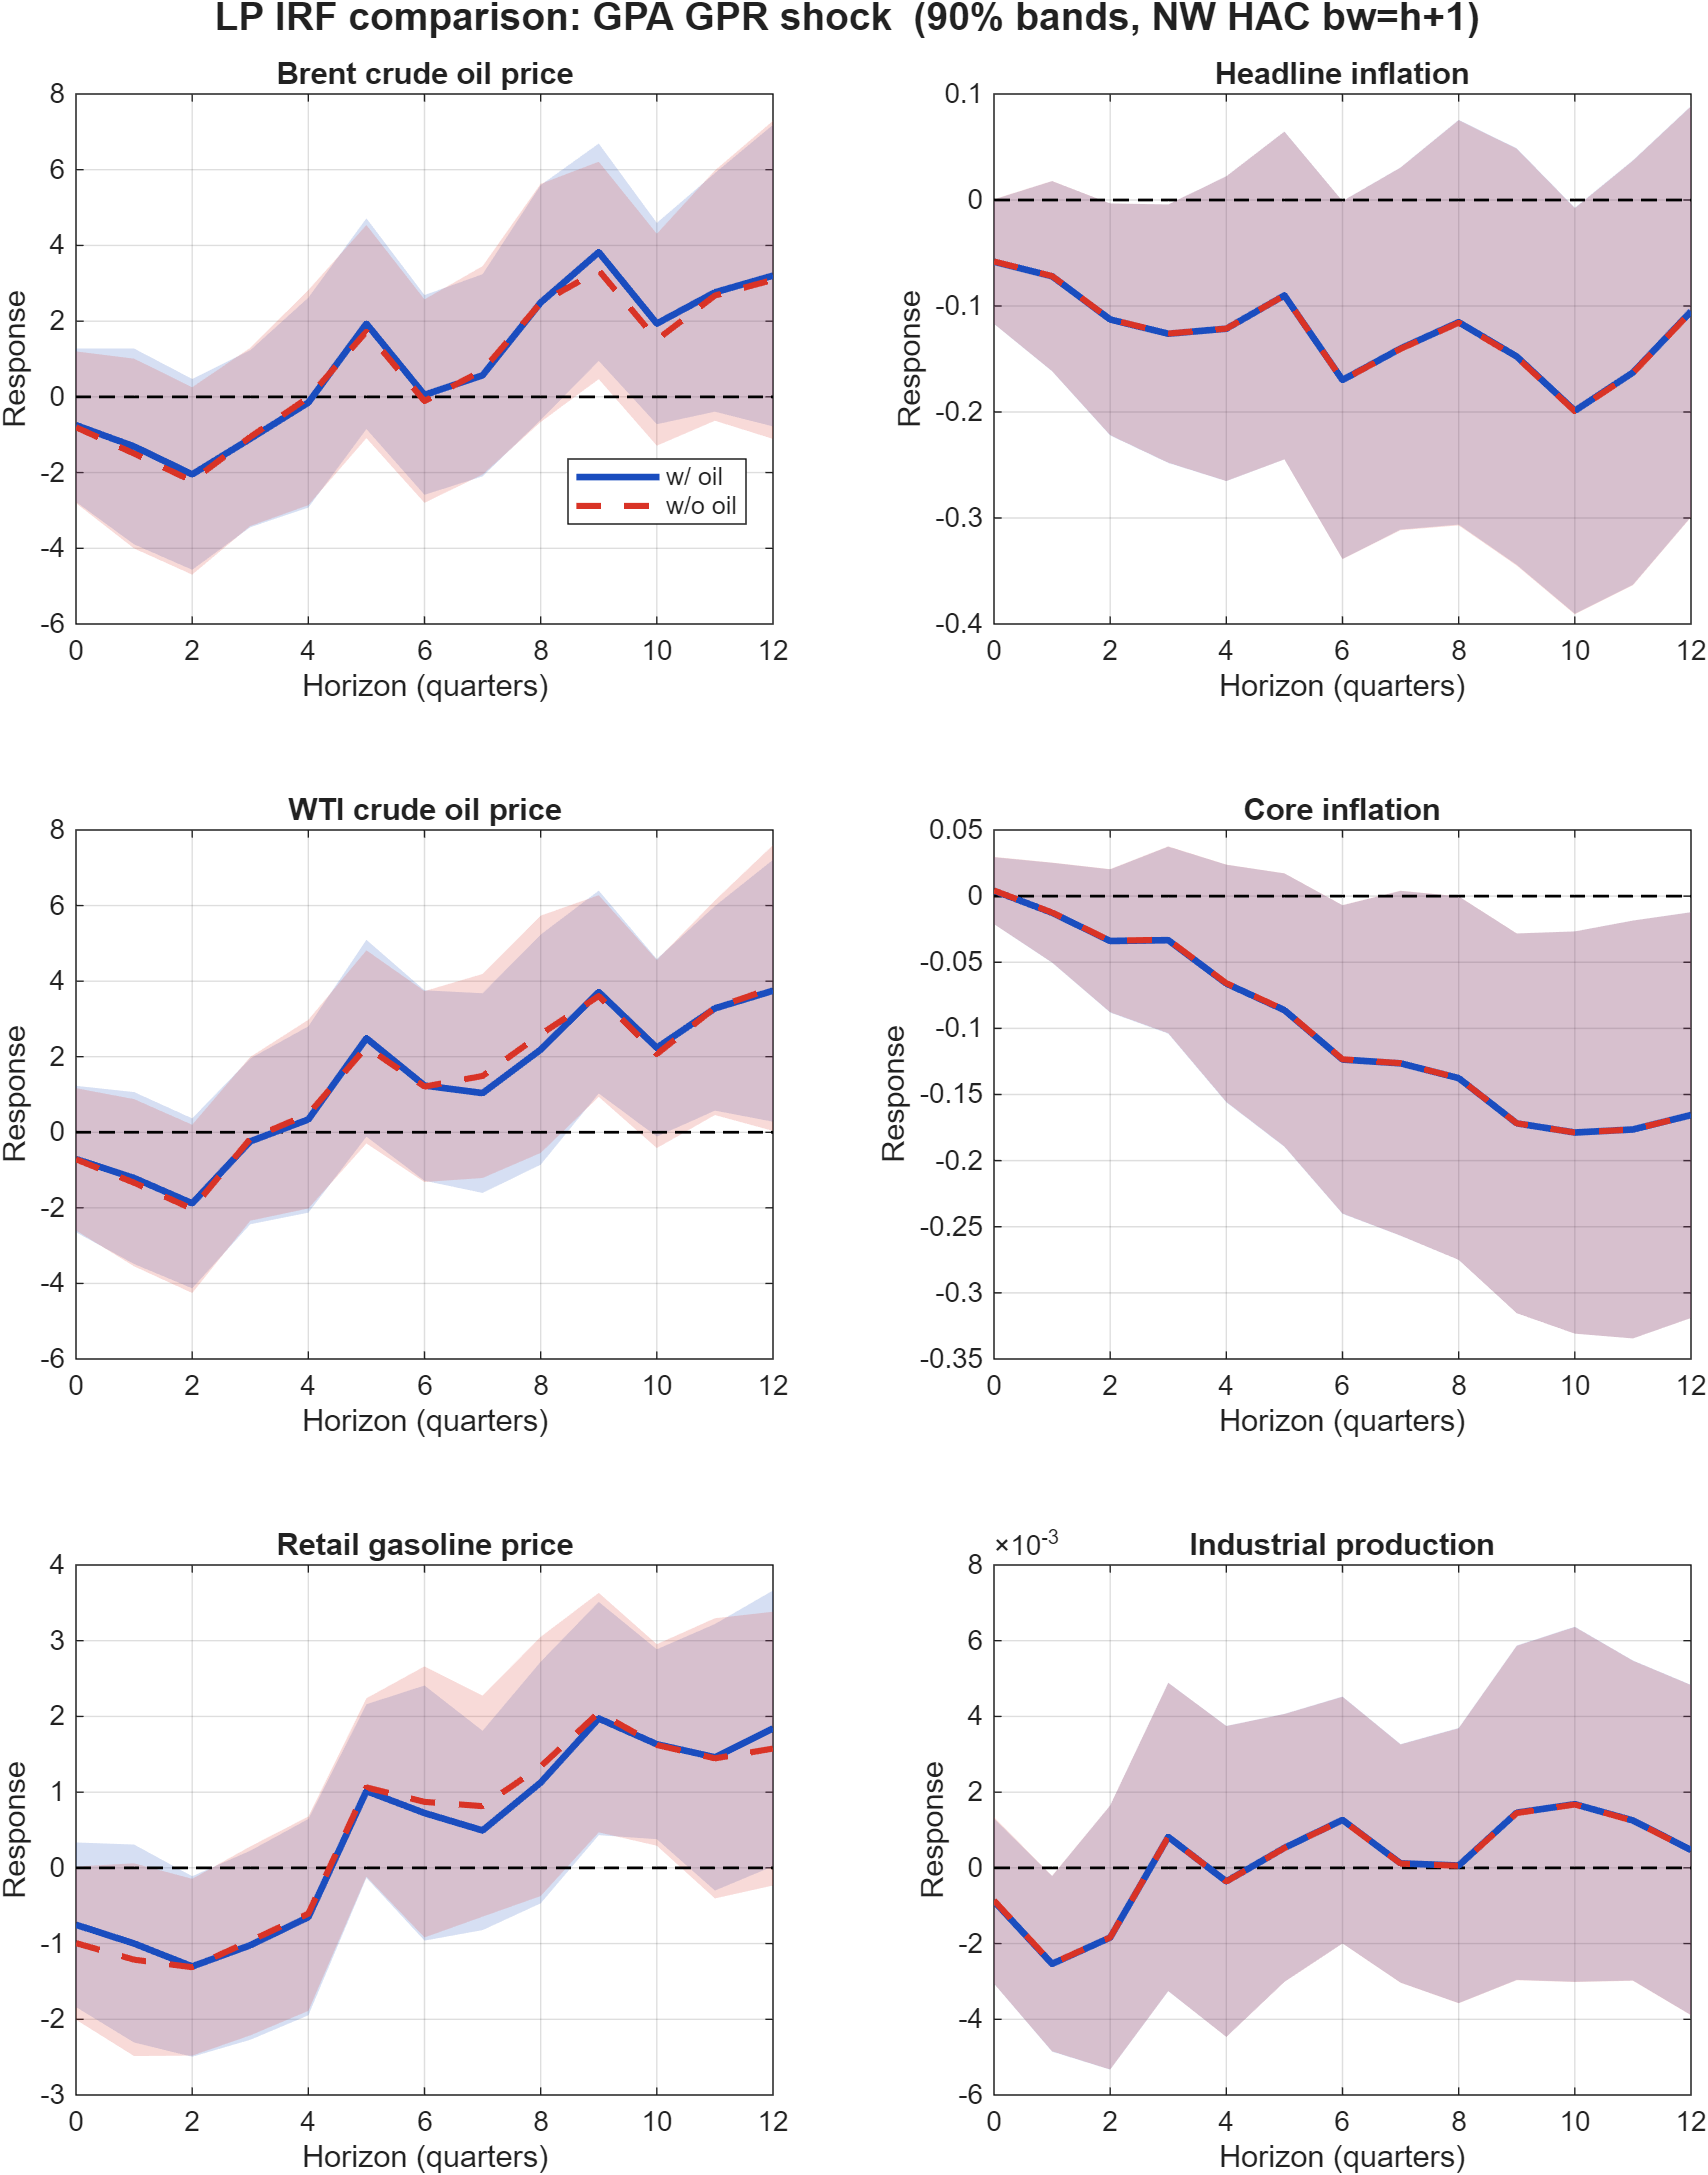
\includegraphics[width=\linewidth]{IRF_compare_GPA.png}
    \caption{IRF to a 1 s.d.\ GPA (acts) shock. Conventions as above.}
    \label{fig:irf_gpa}
\end{figure}

\end{document}
